\documentclass[12pt,a4paper]{article}

\usepackage{fontspec}
\usepackage{polyglossia}
\setmainlanguage{greek}
\setotherlanguage{english}
\setmainfont{DejaVu Serif}
\setsansfont{DejaVu Sans}
\setmonofont{DejaVu Sans Mono}

\usepackage{geometry}
\geometry{left=2.4cm,right=2.4cm,top=2.4cm,bottom=2.5cm}

\usepackage{amsmath,amssymb}
\usepackage{graphicx}
\usepackage{booktabs}
\usepackage{array}
\usepackage{float}
\usepackage{xcolor}
\usepackage{hyperref}
\usepackage{caption}

\hypersetup{
    colorlinks=true,
    linkcolor=blue!55!black,
    urlcolor=blue!55!black
}

\captionsetup{font=small,labelfont=bf}
\setlength{\parindent}{0pt}
\setlength{\parskip}{0.55em}
\renewcommand{\arraystretch}{1.18}

\newcommand{\studentname}{Ρακοβαλής Παύλος}
\newcommand{\studentid}{6931}
\newcommand{\xvalue}{211}

\begin{document}

\begin{titlepage}
    \centering
    \vspace*{2cm}

    {\Large Διοίκηση Συστημάτων Παραγωγής και Υπηρεσιών\par}
    \vspace{0.4cm}
    {\large Ακαδημαϊκό έτος 2025--2026\par}

    \vspace{2.2cm}
    {\Huge \textbf{Αναλυτική Εργασία}\par}

    \vspace{2.2cm}
    \begin{tabular}{rl}
        \textbf{Ονοματεπώνυμο:} & \studentname \\
        \textbf{ΑΕΜ:} & \studentid \\
        \textbf{Αύξων αριθμός εκφώνησης:} & \(x = \xvalue\)
    \end{tabular}

    \vfill
    {\large \today\par}
\end{titlepage}

\tableofcontents
\newpage

\section*{Εισαγωγή}
\addcontentsline{toc}{section}{Εισαγωγή}

Στην παρούσα εργασία επιλύονται οκτώ ασκήσεις της Διοίκησης Συστημάτων Παραγωγής και Υπηρεσιών. Σε όλες τις ασκήσεις χρησιμοποιείται ο αύξων αριθμός \(x = 211\). Οι υπολογισμοί παρουσιάζονται αναλυτικά, ώστε να φαίνεται η μεθοδολογία που εφαρμόστηκε σε κάθε περίπτωση.

\newpage

\section{Άσκηση 1: Ανάλυση κόστους, νεκρό σημείο και επιλογή διαδικασίας}

Δίνεται \(x = 211\). Η τιμή πώλησης των καθισμάτων είναι:
\[
P = 52 + \frac{x}{10} = 52 + \frac{211}{10} = 73{,}10 \text{ €/τεμάχιο}
\]

Τα κόστη των τριών επιλογών είναι:

\begin{table}[H]
\centering
\caption{Κόστη παραγωγής και προμήθειας}
\small
\begin{tabular}{p{2.7cm}p{3.9cm}p{2.7cm}p{4.1cm}}
\toprule
\textbf{Επιλογή} & \textbf{Σταθερό κόστος} & \textbf{Μεταβλητό κόστος} & \textbf{Συνάρτηση κόστους} \\
\midrule
Διαδικασία Α & \(24.000 + 10 \cdot 211 = 26.110\) & 36 & \(C_A(Q)=26.110+36Q\) \\
Διαδικασία Β & \(34.000 + 8 \cdot 211 = 35.688\) & 26 & \(C_B(Q)=35.688+26Q\) \\
Υπεργολάβος & 0 & 44 & \(C_Y(Q)=44Q\) \\
\bottomrule
\end{tabular}
\end{table}

Η συνάρτηση εσόδων είναι:
\[
R(Q)=73{,}10Q
\]

\subsection{Νεκρό σημείο διαδικασιών Α και Β}

Το νεκρό σημείο υπολογίζεται από:
\[
Q_{BE}=\frac{F}{P-v}
\]

Για τη διαδικασία Α:
\[
Q_{BE,A}=\frac{26.110}{73{,}10-36}=\frac{26.110}{37{,}10}=703{,}77
\]
Άρα η ελάχιστη ακέραιη ποσότητα είναι:
\[
Q_{BE,A}=704 \text{ τεμάχια}
\]

Για τη διαδικασία Β:
\[
Q_{BE,B}=\frac{35.688}{73{,}10-26}=\frac{35.688}{47{,}10}=757{,}71
\]
Άρα η ελάχιστη ακέραιη ποσότητα είναι:
\[
Q_{BE,B}=758 \text{ τεμάχια}
\]

\subsection{Προτιμότερη επιλογή παραγωγής ή προμήθειας}

Επειδή η τιμή πώλησης είναι ίδια για όλες τις επιλογές, η προτιμότερη επιλογή είναι εκείνη που έχει το μικρότερο συνολικό κόστος.

Τα σημεία τομής είναι:
\[
26.110+36Q=35.688+26Q \Rightarrow Q=957{,}80
\]
\[
44Q=26.110+36Q \Rightarrow Q=3.263{,}75
\]
\[
44Q=35.688+26Q \Rightarrow Q=1.982{,}67
\]

Επομένως, για ακέραιες ποσότητες:

\begin{table}[H]
\centering
\caption{Προτιμότερη επιλογή ανά περιοχή ζήτησης}
\begin{tabular}{ll}
\toprule
\textbf{Ετήσια ζήτηση} & \textbf{Προτιμότερη επιλογή} \\
\midrule
\(Q \leq 1.982\) & Υπεργολάβος \\
\(Q \geq 1.983\) & Διαδικασία Β \\
\bottomrule
\end{tabular}
\end{table}

Η διαδικασία Α δεν είναι ποτέ η οικονομικά προτιμότερη επιλογή. Για μικρές ποσότητες είναι ακριβότερη από τον υπεργολάβο, ενώ για μεγαλύτερες ποσότητες είναι ακριβότερη από τη διαδικασία Β.

\begin{figure}[H]
\centering
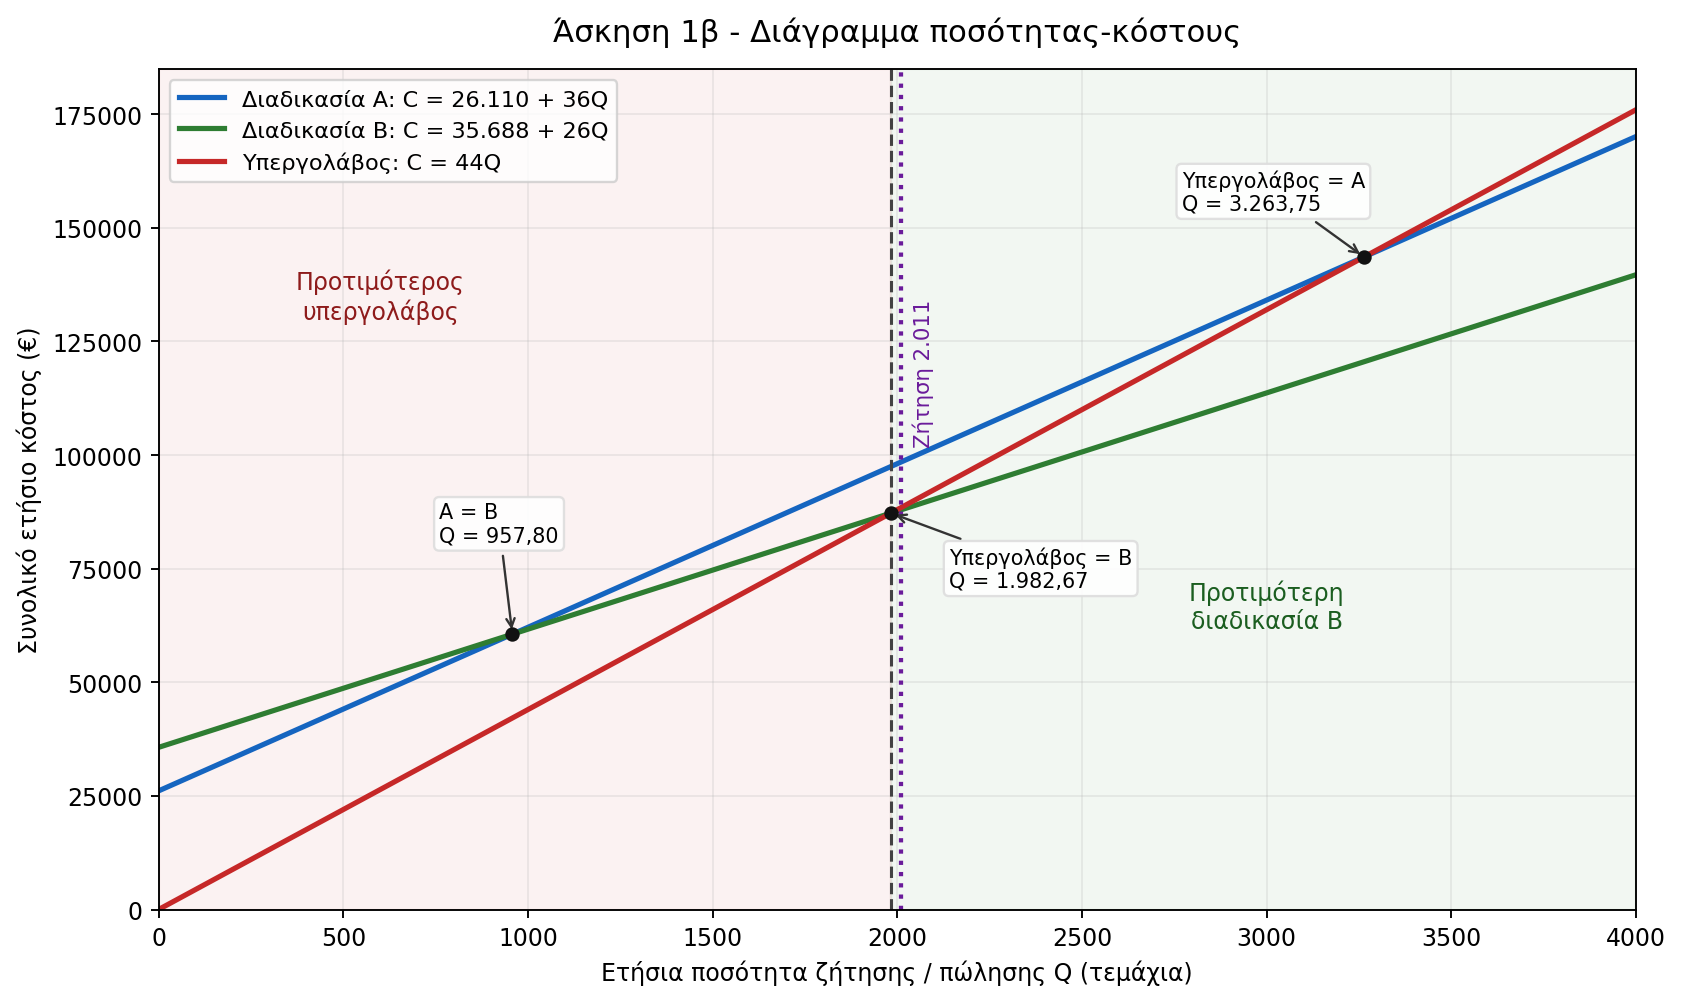
\includegraphics[width=0.95\textwidth]{askisi_1_diagramma_kostous.png}
\caption{Διάγραμμα ποσότητας--κόστους για τις τρεις εναλλακτικές επιλογές}
\end{figure}

\subsection{Κέρδος με επιλογή της διαδικασίας Α}

Η ετήσια ποσότητα πωλήσεων είναι:
\[
Q=1.800+x=1.800+211=2.011 \text{ τεμάχια}
\]

Το ετήσιο κέρδος με τη διαδικασία Α είναι:
\[
\Pi_A=R(Q)-C_A(Q)
\]
\[
R(2.011)=73{,}10 \cdot 2.011=147.004{,}10 \text{ €}
\]
\[
C_A(2.011)=26.110+36 \cdot 2.011=98.506{,}00 \text{ €}
\]
\[
\Pi_A=147.004{,}10-98.506{,}00=48.498{,}10 \text{ €}
\]

\subsection{Αξιολόγηση της επιλογής της διαδικασίας Α}

Για \(Q=2.011\), τα συνολικά κόστη είναι:

\begin{table}[H]
\centering
\caption{Συνολικό κόστος για ζήτηση 2.011 τεμαχίων}
\begin{tabular}{lc}
\toprule
\textbf{Επιλογή} & \textbf{Συνολικό κόστος} \\
\midrule
Διαδικασία Α & 98.506,00 € \\
Διαδικασία Β & 87.974,00 € \\
Υπεργολάβος & 88.484,00 € \\
\bottomrule
\end{tabular}
\end{table}

Η καλύτερη επιλογή είναι η διαδικασία Β. Το ετήσιο κέρδος με τη διαδικασία Β είναι:
\[
\Pi_B=147.004{,}10-87.974{,}00=59.030{,}10 \text{ €}
\]

Άρα η διαδικασία Β δίνει μεγαλύτερο κέρδος από τη διαδικασία Α κατά:
\[
59.030{,}10-48.498{,}10=10.532{,}00 \text{ €}
\]

\section{Άσκηση 2: Μέσος χρόνος ολοκλήρωσης παραγωγής}

Κάθε ξύλινη πολυθρόνα απαιτεί 18 kg ξυλείας. Η εβδομαδιαία ποσότητα ξυλείας είναι:
\[
450+6x=450+6 \cdot 211=1.716 \text{ kg/εβδομάδα}
\]

Ο ρυθμός παραγωγής είναι:
\[
\lambda=\frac{1.716}{18}=95{,}33 \text{ πολυθρόνες/εβδομάδα}
\]

Στο εργοστάσιο υπάρχουν κατά μέσο όρο 120 πολυθρόνες σε διάφορες φάσεις κατασκευής. Με βάση τον νόμο του Little:
\[
WIP=\lambda T
\]
άρα:
\[
T=\frac{WIP}{\lambda}=\frac{120}{95{,}33}=1{,}2587 \text{ εβδομάδες}
\]

Σε ημέρες:
\[
1{,}2587 \cdot 7=8{,}81 \text{ ημέρες}
\]

Επομένως, ο μέσος χρόνος ολοκλήρωσης παραγωγής μίας πολυθρόνας είναι περίπου:
\[
\boxed{1{,}26 \text{ εβδομάδες ή } 8{,}81 \text{ ημέρες}}
\]

\section{Άσκηση 3: Πρότυπο μεταφοράς}

Για \(x=211\), οι δυναμικότητες είναι:
\[
\text{Εργοστάσιο 1}=150
\]
\[
\text{Εργοστάσιο 2}=100+\frac{211}{3}=170{,}33 \simeq 170
\]

Η συνολική δυναμικότητα είναι \(320\) μονάδες. Οι ζητήσεις των αποθηκών είναι:
\[
A=50,\quad B=60,\quad \Gamma=70,\quad \Delta=60+\frac{211}{5}=102{,}20 \simeq 102
\]

Η συνολική ζήτηση είναι:
\[
50+60+70+102=282
\]

Επειδή η δυναμικότητα είναι μεγαλύτερη από τη ζήτηση, προστίθεται εικονική αποθήκη \(E\) με ζήτηση:
\[
320-282=38
\]
και μηδενικό κόστος μεταφοράς.

\begin{table}[H]
\centering
\caption{Ισορροπημένος πίνακας μεταφοράς}
\begin{tabular}{lrrrrrr}
\toprule
 & \textbf{Α} & \textbf{Β} & \textbf{Γ} & \textbf{Δ} & \textbf{Εικονική Ε} & \textbf{Προσφορά} \\
\midrule
Εργοστάσιο 1 & 14 & 20 & 14 & 18 & 0 & 150 \\
Εργοστάσιο 2 & 15 & 18 & 17 & 16 & 0 & 170 \\
\midrule
Ζήτηση & 50 & 60 & 70 & 102 & 38 & 320 \\
\bottomrule
\end{tabular}
\end{table}

\subsection{Αρχική λύση με τη μέθοδο της ΒΔ γωνίας}

\begin{table}[H]
\centering
\caption{Αρχική λύση ΒΔ γωνίας}
\begin{tabular}{lrrrrrr}
\toprule
 & \textbf{Α} & \textbf{Β} & \textbf{Γ} & \textbf{Δ} & \textbf{Εικονική Ε} & \textbf{Προσφορά} \\
\midrule
Εργοστάσιο 1 & 50 & 60 & 40 & 0 & 0 & 150 \\
Εργοστάσιο 2 & 0 & 0 & 30 & 102 & 38 & 170 \\
\midrule
Ζήτηση & 50 & 60 & 70 & 102 & 38 & 320 \\
\bottomrule
\end{tabular}
\end{table}

Το κόστος της αρχικής λύσης είναι:
\[
C=50\cdot14+60\cdot20+40\cdot14+30\cdot17+102\cdot16+38\cdot0=4.602
\]

\subsection{Βελτίωση με MODI}

Με την πρώτη εφαρμογή MODI προκύπτουν αρνητικοί δείκτες βελτίωσης, με πιο αρνητικό τον δείκτη της μεταβλητής \(x_{2B}\). Ο κλειστός βρόχος είναι:
\[
x_{2B}(+),\ x_{2\Gamma}(-),\ x_{1\Gamma}(+),\ x_{1B}(-)
\]
και:
\[
\theta=\min(30,60)=30
\]

Η ενδιάμεση λύση έχει κόστος:
\[
C=50\cdot14+30\cdot20+70\cdot14+30\cdot18+102\cdot16=4.452
\]

Στη δεύτερη εφαρμογή MODI επιλέγεται η μεταβλητή \(x_{1E}\). Ο κλειστός βρόχος είναι:
\[
x_{1E}(+),\ x_{1B}(-),\ x_{2B}(+),\ x_{2E}(-)
\]
και:
\[
\theta=\min(30,38)=30
\]

Η τελική λύση είναι:

\begin{table}[H]
\centering
\caption{Βέλτιστη λύση μεταφοράς}
\begin{tabular}{lrrrrrr}
\toprule
 & \textbf{Α} & \textbf{Β} & \textbf{Γ} & \textbf{Δ} & \textbf{Εικονική Ε} & \textbf{Προσφορά} \\
\midrule
Εργοστάσιο 1 & 50 & 0 & 70 & 0 & 30 & 150 \\
Εργοστάσιο 2 & 0 & 60 & 0 & 102 & 8 & 170 \\
\midrule
Ζήτηση & 50 & 60 & 70 & 102 & 38 & 320 \\
\bottomrule
\end{tabular}
\end{table}

Το ελάχιστο μηνιαίο κόστος μεταφοράς είναι:
\[
C_{\min}=50\cdot14+70\cdot14+60\cdot18+102\cdot16=4.392
\]

\section{Άσκηση 4: Δυναμικότητα κυψέλης παραγωγής}

Οι χρόνοι εργασίας είναι:

\begin{table}[H]
\centering
\caption{Χρόνοι εργασίας ανά μηχανή}
\begin{tabular}{lc}
\toprule
\textbf{Μηχανή} & \textbf{Χρόνος εργασίας} \\
\midrule
Μ1 & 180 sec \\
Μ2 & 240 sec \\
Μ3 & 300 sec \\
Μ4 & \(50+x=261\) sec \\
\bottomrule
\end{tabular}
\end{table}

Οι δυναμικότητες των μηχανών είναι:
\[
M1:\frac{3.600}{180}=20,\quad
M2:\frac{3.600}{240}=15,\quad
M3:\frac{3.600}{300}=12,\quad
M4:\frac{3.600}{261}=13{,}79
\]

Η μικρότερη δυναμικότητα είναι της Μ3. Άρα:
\[
\boxed{\text{Δυναμικότητα κυψέλης}=12 \text{ μονάδες/ώρα}}
\]
και το σημείο συμφόρησης είναι η Μ3.

Για ζήτηση 10 μονάδων ανά ώρα, ο ενδεδειγμένος ρυθμός παραγωγής είναι 10 μονάδες ανά ώρα, αφού \(10<12\). Ο χρονικός κύκλος είναι:
\[
CT=\frac{3.600}{10}=360 \text{ sec/μονάδα}
\]

\begin{table}[H]
\centering
\caption{Χρησιμοποίηση και νεκροί χρόνοι}
\begin{tabular}{lccc}
\toprule
\textbf{Μηχανή} & \textbf{Χρόνος εργασίας} & \textbf{Χρησιμοποίηση} & \textbf{Νεκρός χρόνος} \\
\midrule
Μ1 & 180 & \(180/360=50{,}00\%\) & 180 sec \\
Μ2 & 240 & \(240/360=66{,}67\%\) & 120 sec \\
Μ3 & 300 & \(300/360=83{,}33\%\) & 60 sec \\
Μ4 & 261 & \(261/360=72{,}50\%\) & 99 sec \\
\bottomrule
\end{tabular}
\end{table}

Η κυψέλη μπορεί να καλύψει αύξηση της ζήτησης μέχρι τη δυναμικότητά της, δηλαδή μέχρι 12 μονάδες ανά ώρα. Το μέγιστο ποσοστό αύξησης είναι:
\[
\frac{12-10}{10}\cdot100\%=20\%
\]

\section{Άσκηση 5: Εξισορρόπηση γραμμής συναρμολόγησης}

Με \(x=211\), οι χρόνοι εργασιών μετά τη στρογγυλοποίηση είναι:

\begin{table}[H]
\centering
\caption{Διάρκειες εργασιών}
\begin{tabular}{llcc}
\toprule
\textbf{Εργασία} & \textbf{Προαπαιτούμενες} & \textbf{Υπολογισμός} & \textbf{Διάρκεια} \\
\midrule
A & Καμία & \(35+211/9=58{,}44\) & 58 sec \\
B & A & 24 & 24 sec \\
C & A & 32 & 32 sec \\
D & B & 43 & 43 sec \\
E & C, D & \(12+211/11=31{,}18\) & 31 sec \\
F & E & \(20+211/11=39{,}18\) & 39 sec \\
\bottomrule
\end{tabular}
\end{table}

Οι τεχνολογικοί περιορισμοί είναι:
\[
A \rightarrow B \rightarrow D \rightarrow E \rightarrow F
\]
\[
A \rightarrow C \rightarrow E \rightarrow F
\]

\begin{figure}[H]
\centering
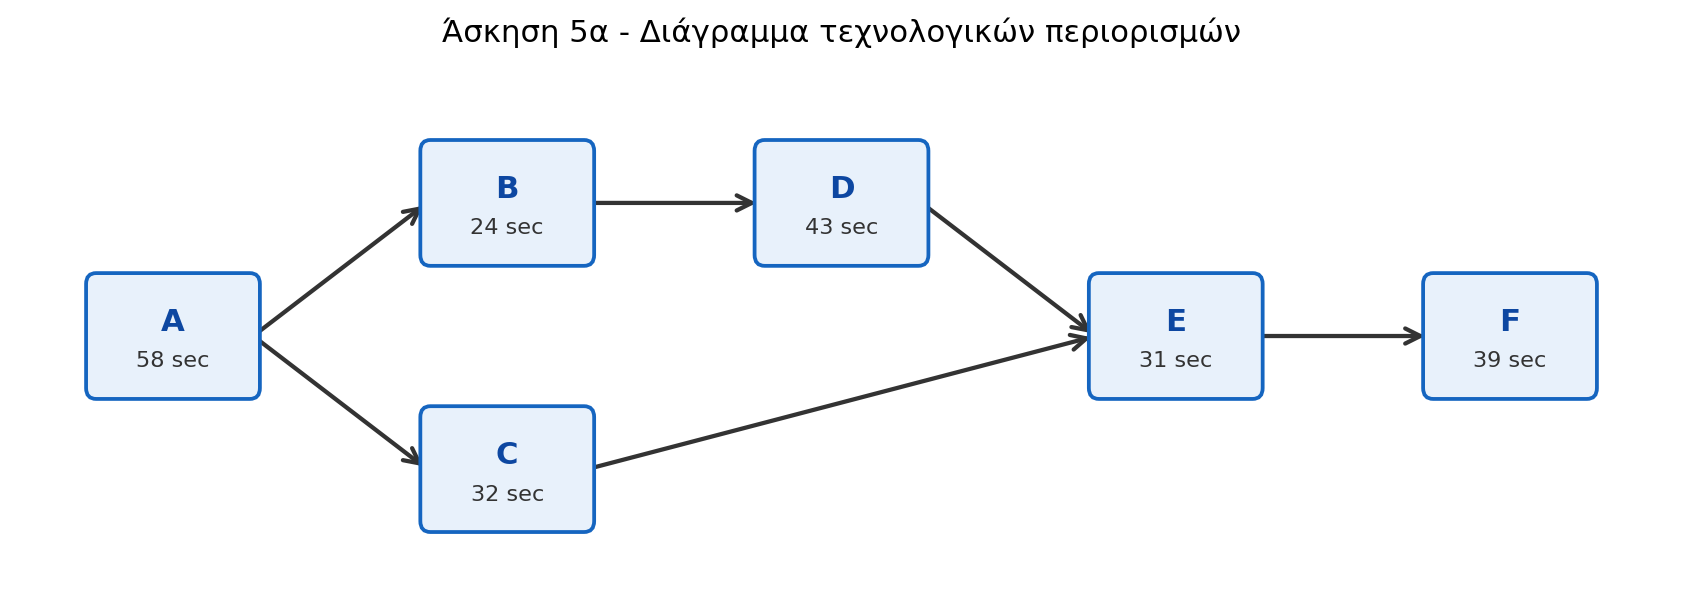
\includegraphics[width=0.95\textwidth]{askisi_5_diagramma_texnologikon_periorismon.png}
\caption{Διάγραμμα τεχνολογικών περιορισμών}
\end{figure}

Ο επιθυμητός ρυθμός παραγωγής είναι 40 μονάδες ανά ώρα, άρα ο χρονικός κύκλος είναι:
\[
C=\frac{3.600}{40}=90 \text{ sec/μονάδα}
\]

Το συνολικό περιεχόμενο εργασίας είναι:
\[
\sum t_i=58+24+32+43+31+39=227 \text{ sec}
\]

Ο θεωρητικά ελάχιστος αριθμός σταθμών είναι:
\[
N_{\min}=\left\lceil \frac{227}{90} \right\rceil=3
\]

Μία εφικτή κατανομή είναι:

\begin{table}[H]
\centering
\caption{Κατανομή εργασιών σε σταθμούς}
\begin{tabular}{llcc}
\toprule
\textbf{Σταθμός} & \textbf{Εργασίες} & \textbf{Χρόνος σταθμού} & \textbf{Νεκρός χρόνος} \\
\midrule
1 & A, B & \(58+24=82\) sec & 8 sec \\
2 & C, D & \(32+43=75\) sec & 15 sec \\
3 & E, F & \(31+39=70\) sec & 20 sec \\
\bottomrule
\end{tabular}
\end{table}

Η αποδοτικότητα της γραμμής είναι:
\[
E=\frac{227}{3\cdot90}=0{,}8407=84{,}07\%
\]

Ο δείκτης ομαλότητας, με βάση τον μεγαλύτερο χρόνο σταθμού \(ST_{\max}=82\), είναι:
\[
SI=\sqrt{(82-82)^2+(82-75)^2+(82-70)^2}
=\sqrt{193}=13{,}89 \text{ sec}
\]

\section{Άσκηση 6: Απλή εκθετική εξομάλυνση}

Με \(x=211\), οι τιμές που περιέχουν τον αύξοντα αριθμό γίνονται:
\[
280-\frac{211}{4}=227{,}25\simeq227
\]
\[
145+\frac{211}{2}=250{,}50\simeq251
\]
\[
150+\frac{211}{5}=192{,}20\simeq192
\]
\[
267-\frac{211}{4}=214{,}25\simeq214
\]

Η ζήτηση των 24 μηνών είναι:

\begin{table}[H]
\centering
\caption{Ζήτηση 24 μηνών}
\begin{tabular}{rrrrrrrrrrrr}
\toprule
1 & 2 & 3 & 4 & 5 & 6 & 7 & 8 & 9 & 10 & 11 & 12 \\
\midrule
227 & 250 & 218 & 180 & 192 & 205 & 188 & 235 & 190 & 187 & 251 & 275 \\
\midrule
13 & 14 & 15 & 16 & 17 & 18 & 19 & 20 & 21 & 22 & 23 & 24 \\
\midrule
192 & 226 & 200 & 173 & 232 & 299 & 173 & 209 & 264 & 203 & 214 & 266 \\
\bottomrule
\end{tabular}
\end{table}

Η αρχική εκτίμηση στο τέλος του μήνα 11 είναι:
\[
\begin{aligned}
F_{12} &= \frac{\sum_{t=1}^{11} A_t}{11} \\
       &= \frac{2.323}{11}=211{,}18
\end{aligned}
\]

Ο τύπος της απλής εκθετικής εξομάλυνσης είναι:
\[
F_{t+1}=\alpha A_t+(1-\alpha)F_t
\]

Η ακρίβεια των προβλέψεων για τους μήνες 13 έως 24 συγκρίνεται για \(\alpha=0{,}1\) και \(\alpha=0{,}2\).

\begin{table}[H]
\centering
\caption{Σύγκριση ακρίβειας εκθετικής εξομάλυνσης}
\begin{tabular}{lccc}
\toprule
\(\alpha\) & \textbf{MAD} & \textbf{MSE} & \textbf{MAPE} \\
\midrule
0,1 & 31,34 & 1.502,33 & 13,91\% \\
0,2 & 33,63 & 1.642,75 & 15,12\% \\
\bottomrule
\end{tabular}
\end{table}

Το \(\alpha=0{,}1\) έχει μικρότερα σφάλματα και επιλέγεται.

Με \(\alpha=0{,}1\), η πρόβλεψη για τον μήνα 25 είναι:
\[
F_{25}=0{,}1\cdot266+0{,}9\cdot218{,}23=223{,}01
\]

Στην απλή εκθετική εξομάλυνση, χωρίς νέα πραγματικά δεδομένα, οι προβλέψεις για περισσότερες μελλοντικές περιόδους παραμένουν ίδιες. Άρα:
\[
F_{25}=F_{26}=\cdots=F_{36}=223{,}01
\]

Στρογγυλοποιημένα:
\[
\boxed{F_{25}=F_{26}=\cdots=F_{36}=223 \text{ μονάδες}}
\]

\section{Άσκηση 7: Σύστημα EOQ}

Τα δεδομένα είναι:
\[
d=80 \text{ μονάδες/εβδομάδα}
\]
\[
D=80\cdot52=4.160 \text{ μονάδες/έτος}
\]
\[
L=1 \text{ εβδομάδα}
\]
\[
S=50+x=261 \text{ €/παραγγελία}
\]
\[
Q=100+x=311 \text{ μονάδες}
\]

\subsection{Στάθμη παραγγελίας}

Χωρίς απόθεμα ασφαλείας:
\[
ROP=dL=80\cdot1=80 \text{ μονάδες}
\]

\subsection{Μέσο απόθεμα και λοιποί δείκτες}

Το μέσο απόθεμα είναι:
\[
I_{\text{μέσο}}=\frac{Q}{2}=\frac{311}{2}=155{,}5 \text{ μονάδες}
\]

Ο χρόνος μεταξύ διαδοχικών παραγγελιών είναι:
\[
T=\frac{Q}{d}=\frac{311}{80}=3{,}8875 \text{ εβδομάδες}
\]

Ο αριθμός παραγγελιών ανά έτος είναι:
\[
N=\frac{D}{Q}=\frac{4.160}{311}=13{,}38
\]

Η κυκλοφοριακή ταχύτητα αποθεμάτων είναι:
\[
\frac{D}{I_{\text{μέσο}}}=\frac{4.160}{155{,}5}=26{,}75 \text{ φορές/έτος}
\]

Η διάρκεια αποθεμάτων είναι:
\[
\frac{155{,}5}{80}=1{,}94 \text{ εβδομάδες}
\]

\subsection{Ετήσιο κόστος}

Το ετήσιο κόστος παραγγελιών είναι:
\[
\frac{D}{Q}S=\frac{4.160}{311}\cdot261=3.491{,}19 \text{ €}
\]

Επειδή το \(Q=311\) είναι η βέλτιστη ποσότητα EOQ, στο άριστο σημείο το ετήσιο κόστος παραγγελιών είναι ίσο με το ετήσιο κόστος διατήρησης:
\[
C_H=3.491{,}19 \text{ €}
\]

Το συνολικό ετήσιο κόστος είναι:
\[
TC=3.491{,}19+3.491{,}19=6.982{,}38 \text{ €}
\]

\subsection{Κόστος διατήρησης ανά μονάδα}

Από τον τύπο EOQ:
\[
Q=\sqrt{\frac{2DS}{H}}
\]
οπότε:
\[
H=\frac{2DS}{Q^2}
\]

Άρα:
\[
H=\frac{2\cdot4.160\cdot261}{311^2}
=\frac{2.171.520}{96.721}=22{,}45 \text{ €/μονάδα/έτος}
\]

\section{Άσκηση 8: Ικανότητα διαδικασίας και διάγραμμα ελέγχου}

Η ονομαστική τιμή είναι \(1000\) ml και οι προδιαγραφές είναι \(1000\pm10\) ml. Άρα:
\[
LSL=990,\quad USL=1010
\]

Η τυπική απόκλιση είναι:
\[
\sigma=\frac{x}{50}=\frac{211}{50}=4{,}22 \text{ ml}
\]

\subsection{Φυσικά όρια ανοχών και δείκτης ικανότητας}

Τα φυσικά όρια ανοχών είναι:
\[
\mu\pm3\sigma=1000\pm3\cdot4{,}22=1000\pm12{,}66
\]
\[
\text{Κάτω φυσικό όριο}=987{,}34 \text{ ml}
\]
\[
\text{Άνω φυσικό όριο}=1012{,}66 \text{ ml}
\]

Ο δείκτης ικανότητας είναι:
\[
C_p=\frac{USL-LSL}{6\sigma}
=\frac{1010-990}{6\cdot4{,}22}
=\frac{20}{25{,}32}=0{,}79
\]

Επειδή \(C_p<1\), η διαδικασία δεν είναι ικανή να ανταποκριθεί στις ποιοτικές απαιτήσεις. Τα φυσικά όρια ανοχών είναι ευρύτερα από τα όρια προδιαγραφών.

\subsection{Διάγραμμα ελέγχου μέσης τιμής}

Για δείγματα μεγέθους \(n=5\):
\[
\sigma_{\bar{x}}=\frac{\sigma}{\sqrt{n}}=\frac{4{,}22}{\sqrt{5}}=1{,}8872 \text{ ml}
\]

Τα όρια ελέγχου τριών τυπικών αποκλίσεων είναι:
\[
UCL=1000+3\cdot1{,}8872=1005{,}66
\]
\[
CL=1000{,}00
\]
\[
LCL=1000-3\cdot1{,}8872=994{,}34
\]

\begin{figure}[H]
\centering
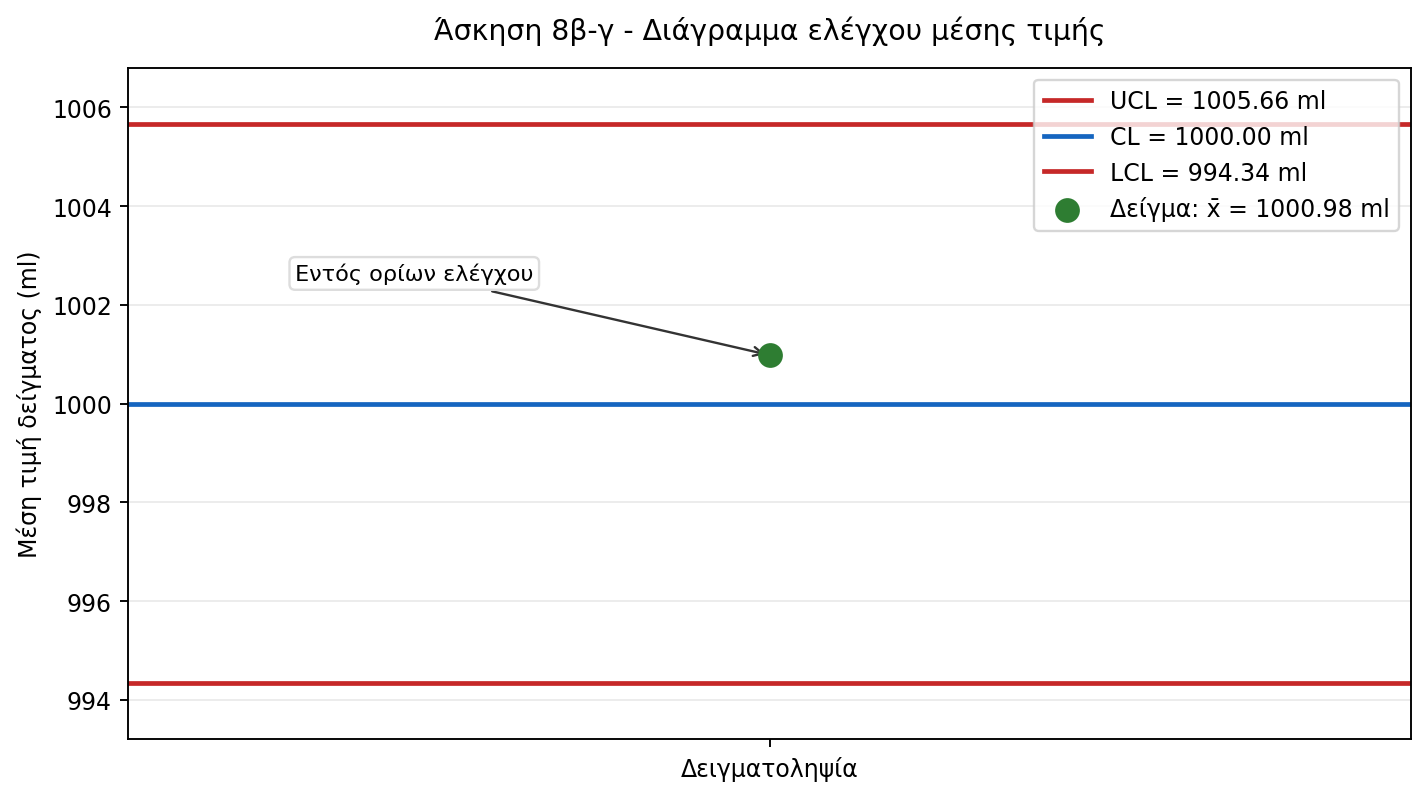
\includegraphics[width=0.85\textwidth]{askisi_8_diagramma_elegxou_meshs_timis.png}
\caption{Διάγραμμα ελέγχου μέσης τιμής}
\end{figure}

\subsection{Έλεγχος δείγματος}

Το δείγμα είναι:
\[
1000{,}3,\quad 1000{,}8,\quad 1000{,}0,\quad 1001{,}7,\quad 1000+\frac{211}{100}=1002{,}11
\]

Η μέση τιμή του δείγματος είναι:
\[
\bar{x}=\frac{1000{,}3+1000{,}8+1000{,}0+1001{,}7+1002{,}11}{5}
=1000{,}982 \text{ ml}
\]

Επειδή:
\[
994{,}34 < 1000{,}982 < 1005{,}66
\]
το αποτέλεσμα βρίσκεται εντός των ορίων ελέγχου. Συνεπώς, δεν υπάρχει ένδειξη ότι η διαδικασία εμφιάλωσης ήταν εκτός στατιστικού ελέγχου κατά τη στιγμή της δειγματοληψίας.

\section*{Συμπεράσματα}
\addcontentsline{toc}{section}{Συμπεράσματα}

Με βάση τους υπολογισμούς, στην πρώτη άσκηση η διαδικασία Β είναι η καλύτερη επιλογή για τη ζήτηση των 2.011 τεμαχίων, ενώ η διαδικασία Α δεν είναι ποτέ η φθηνότερη εναλλακτική. Στις ασκήσεις παραγωγικής ροής, η κυψέλη της άσκησης 4 έχει δυναμικότητα 12 μονάδες ανά ώρα και μπορεί να καλύψει αύξηση ζήτησης έως 20\%. Στην εξισορρόπηση της γραμμής συναρμολόγησης επιτυγχάνεται εφικτή λύση με 3 σταθμούς και αποδοτικότητα 84,07\%. Στην πρόβλεψη ζήτησης επιλέγεται η σταθερά εξομάλυνσης \(\alpha=0{,}1\), ενώ στο EOQ προκύπτει συνολικό ετήσιο κόστος 6.982,38 €. Τέλος, στην άσκηση στατιστικού ελέγχου η διαδικασία είναι στατιστικά υπό έλεγχο για το δοθέν δείγμα, αλλά δεν είναι ικανή ως προς τις προδιαγραφές επειδή \(C_p=0{,}79<1\).

\end{document}
